\documentclass[12pt,twoside]{report}

\usepackage[utf8]{inputenc}
\usepackage[brazil]{babel}
\usepackage{csquotes}
\usepackage{graphicx}
\usepackage[a4paper,width=150mm,top=25mm,bottom=25mm,bindingoffset=6mm]{geometry}
\usepackage{fancyhdr}
\usepackage[backend=bibtex,sorting=none,citestyle=numeric-comp]{biblatex}
\usepackage{mathtools}


% PRE CONFIGURATIONS

\graphicspath{{images/}}
\addbibresource{references.bib}
\setlength{\headheight}{14.5pt}
\pagestyle{fancy}
\fancyhead[RO,LE]{}
\bibliography{references}


\renewcommand{\figurename}{\small Figure}
\newcommand{\figureref}[1]{Fig. \ref{fig:#1}}
\newcommand{\equationref}[1]{Eq. \ref{eq:#1}}
\newcommand{\captiontext}[1]{\footnotesize{#1}}
\newcommand{\code}[1]{\texttt{#1}}


%GLOBAL DEFINITIONS

\gdef\papertitle{Aprendizagem de Máquina\\\normalsize Projeto de Graduação, 2014-2}
\gdef\universityname{Universidade Federal de Pernambuco}
\gdef\centername{Centro de Informática}
\gdef\authorname{Eduardo M. B. de A. Tenório\\Hélio de M. Lins Neto\\Hugo B. Barbosa}


\title{
    {
\includegraphics{ufpelogo.png}}
    \\
    {\large \universityname}
    \\
    {\large \centername}
    \vfill
    \textbf{\papertitle}
    \vfill
}
\author{\authorname}
\date{\normalsize\vfill \today}


\begin{document}
\maketitle

\chapter*{Introdução}

O projeto consiste em gerar 300 amostras a partir de distribuições gaussianas
bivariadas, formando 2 classes. A classe 1 é dividida nas subclasses 1-1 e 1-2,
com 100 amostras cada, e a classe 2 também com 100 amostras. As funções geradoras
possuem os seguintes parâmetros:

\begin{enumerate}
    \item Classe 1-1: $\mu_1 = 60$, $\mu_2 = 30$, $\sigma_1^2 = 9$ e $\sigma_2^2 = 144$
    \item Classe 1-2: $\mu_1 = 52$, $\mu_2 = 30$, $\sigma_1^2 = 9$ e $\sigma_2^2 = 9$
    \item Classe 2: $\mu_1 = 45$, $\mu_2 = 22$, $\sigma_1^2 = 100$ e $\sigma_2^2 = 9$
\end{enumerate}

Os dados são gerados pelas funções \code{mvnrnd} de MATLAB e \code{multivariate\_normal}
do pacote \code{random} de NumPy (biblioteca numérica para Python) e registrados
em arquivos texto de acordo com a regra:

\begin{enumerate}\itemsep0pt
    \item Classe 1-1: \emph{r11.txt}
    \item Classe 1-2: \emph{r12.txt}
    \item Classe 2: \emph{r2.txt}
\end{enumerate}

\noindent Cada linha corresponde a uma amostra, composta por dois números reais
representando a primeira e a segunda variáveis.


\chapter*{Questão 1}

O algoritmo FCM-DFCV foi retirado de \autocite{carvalho.tenorio.cavalcanti.2006},
implementado utilizando Python3.4 com a biblioteca NumPy. A biblioteca matplotlib
foi utilizada para gerar os gráficos necessários para a visualização dos dados e
da classificação final.

Ocorreram poucas dificuldades, entre elas a falta de familiaridade com a biblioteca
NumPy e o entendimento do algoritmo em si. A implementação alcançou protótipos
muito parecidos com a média das distribuições 1-1, 1-2 e 2, obtendo um índice de
Rand entre 55\% e 70\% dependendo da distribuição. Em grande parte das vezes o
algoritmo converge antes de 150 iterações. A seguir são mostrados os dados originais
(\figureref{questao1_original}) e agrupados utilizando Fuzzy c-Means (FCM)
(\figureref{questao1_clusters}).

\begin{figure}[ht]
    \centering
    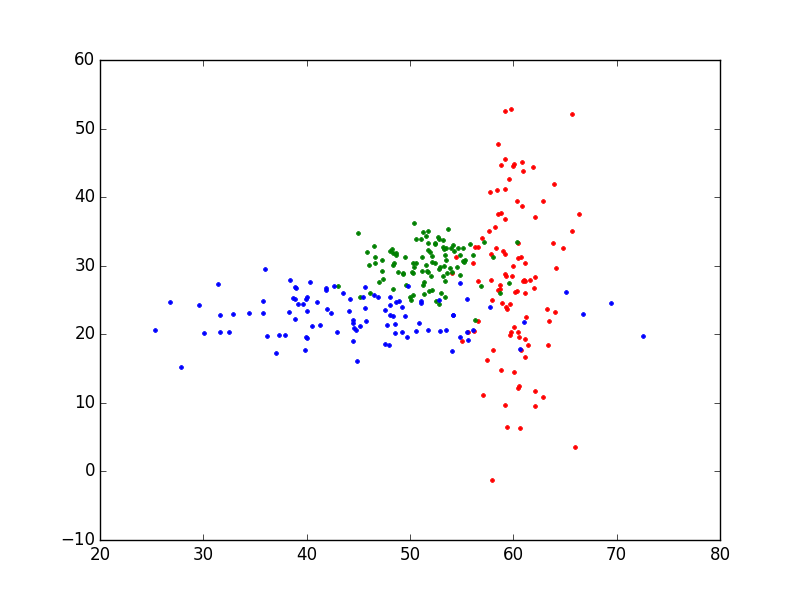
\includegraphics[scale=0.75]{questao1_original}
    \caption{\captiontext{Originais. Classes 1 (1-1 em vermelho e 1-2 em verde) e 2 (azul).}}
    \label{fig:questao1_original}
\end{figure}

\newpage

\begin{figure}[ht]
    \centering
    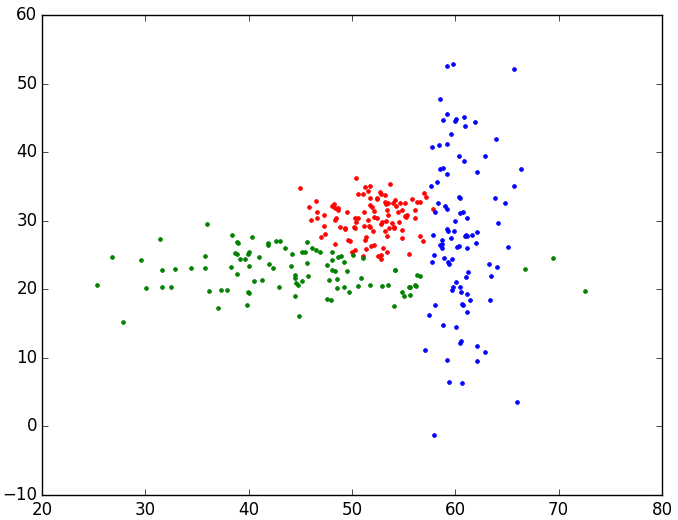
\includegraphics[scale=0.75]{questao1_clusters}
    \caption{\captiontext{FCM. Classes 1 (1-1 em azul e 1-2 em vermelho) e 2 (verde).}}
    \label{fig:questao1_clusters}
\end{figure}


\chapter*{Questão 2}

As probabilidades a priori $P(\omega_1)$ e $P(\omega_2)$ são determinadas pela
maximização da verossimilhança. Neste caso correspondem à razão entre a quantidade
de objetos da classe e do conjunto universo:

\begin{equation}
\begin{split}
P(\omega_1) = \frac{200}{300} = \frac{2}{3}\\\\
P(\omega_2) = \frac{100}{300} = \frac{1}{3}
\end{split}
\label{eq:prob_priori}
\end{equation}


\section*{Letra A}

Para a gaussiana bivariada o método da Estimação da Máxima Verossimilhança
(Maximum Likelihood Estimation, MLE) nos diz que a média e a matrix de covariância
são dadas por

\begin{equation}
\mathbf{\mu} = \frac{1}{N} \sum_{k=1}^N \mathbf{x}_k
\label{eq:letra_a_mean}
\end{equation}

\begin{equation}
\mathbf{\Sigma} = \frac{1}{N} \sum_{k=1}^N (\mathbf{x}_k - \mathbf{\mu})(\mathbf{x}_k - \mathbf{\mu})'
\label{eq:letra_a_covariance}
\end{equation}

\noindent respectivamente, cuja implementação encontra-se em \code{segunda\_a.m}.
A densidade de probabilidade para a classe 2 encontra-se em \figureref{pdf_mle_c2}.
Para a classe 1 o algoritmo Expectation-Maximization (EM) estima um média e uma
matriz de covariância para cada gaussiana da mistura. A descrição do processo
encontra-se no arquivo \code{EM\_GM.m}, com alguns resultados em \figureref{pdf_em_c11}
e \figureref{pdf_em_c12}.

Agora podemos calcular a densidade de probabilidade total da classe 1, ponderando
os valores das subclasses (obtidos pelo EM) e misturando as gaussianas. O resultado
é mostrado em \figureref{pdf_em_c1}.

Por fim, $P(\omega_i|\mathbf{x}_k)$ é calculado a partir dos parâmetros já
encontrados, exibida em \figureref{bayes_c1} e \figureref{bayes_c2}.

\begin{figure}[ht]
    \centering
    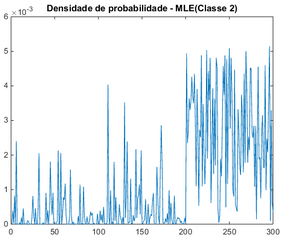
\includegraphics[scale=0.85]{pdf_mle_c2}
    \caption{}
    \label{fig:pdf_mle_c2}
\end{figure}

\begin{figure}[ht]
    \centering
    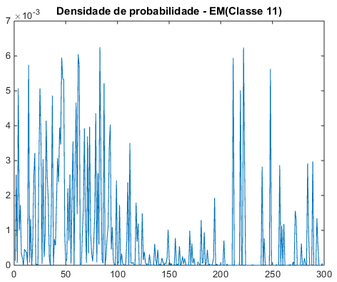
\includegraphics[scale=0.75]{pdf_em_c11}
    \caption{}
    \label{fig:pdf_em_c11}
\end{figure}

\begin{figure}[ht]
    \centering
    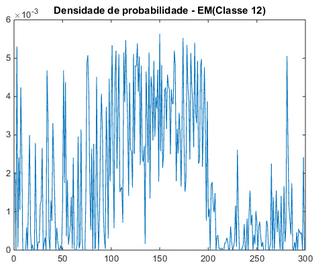
\includegraphics[scale=0.75]{pdf_em_c12}
    \caption{}
    \label{fig:pdf_em_c12}
\end{figure}

\begin{figure}[ht]
    \centering
    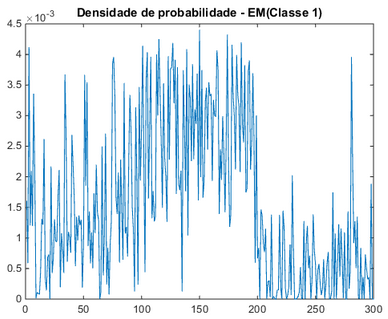
\includegraphics[scale=0.75]{pdf_em_c1}
    \caption{}
    \label{fig:pdf_em_c1}
\end{figure}

\begin{figure}[ht]
    \centering
    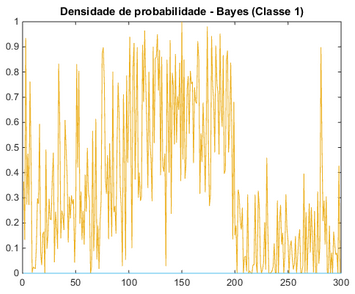
\includegraphics[scale=0.75]{bayes_c1}
    \caption{}
    \label{fig:bayes_c1}
\end{figure}

\begin{figure}[ht]
    \centering
    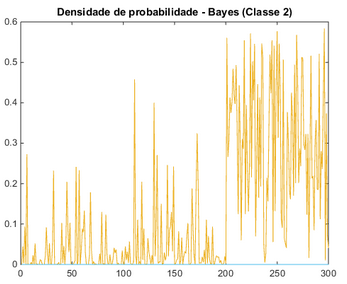
\includegraphics[scale=0.75]{bayes_c2}
    \caption{}
    \label{fig:bayes_c2}
\end{figure}


\section*{Letra B}

Utilizando a função de kernel bivariada, os códigos \code{parzen.m}, \code{bivar.m},
\code{multi.m} e \code{uni.m} implementam a Janela de Parzen e definem as densidades
de probabilidade variando o valor de h (figuras abaixo). A partir destes resultados
é possível calcular $P(\omega_i|\mathbf{x}_k)$, esboçado em \figureref{parzen_c2_h06}.

\begin{figure}[ht]
    \centering
    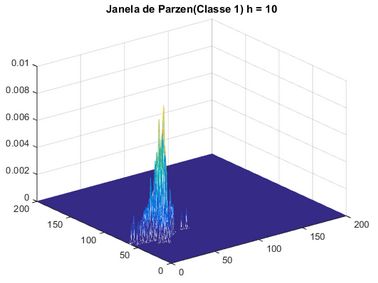
\includegraphics[scale=0.75]{parzen_c1_h10}
    \caption{}
    \label{fig:parzen_c1_h10}
\end{figure}

\begin{figure}[ht]
    \centering
    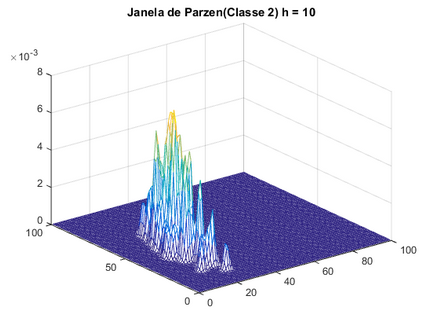
\includegraphics[scale=0.75]{parzen_c2_h10}
    \caption{}
    \label{fig:parzen_c2_h10}
\end{figure}

\begin{figure}[ht]
    \centering
    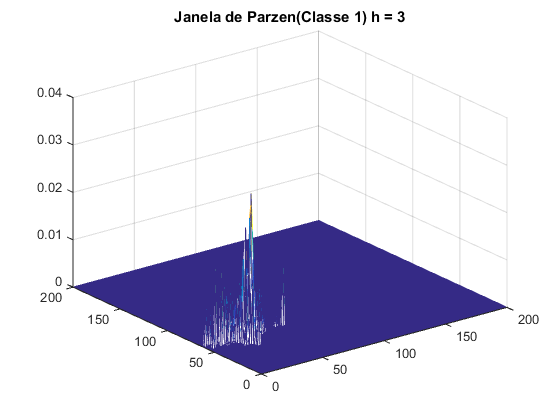
\includegraphics[scale=0.75]{parzen_c1_h3}
    \caption{}
    \label{fig:parzen_c1_h3}
\end{figure}

\begin{figure}[ht]
    \centering
    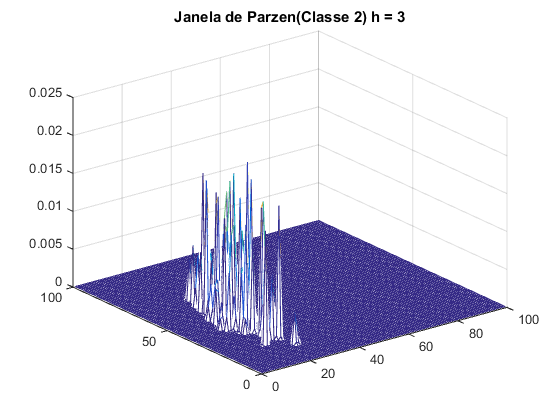
\includegraphics[scale=0.75]{parzen_c2_h3}
    \caption{}
    \label{fig:parzen_c2_h3}
\end{figure}

\begin{figure}[ht]
    \centering
    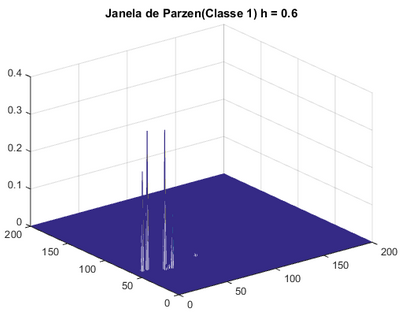
\includegraphics[scale=0.75]{parzen_c1_h06}
    \caption{}
    \label{fig:parzen_c1_h06}
\end{figure}

\begin{figure}[ht]
    \centering
    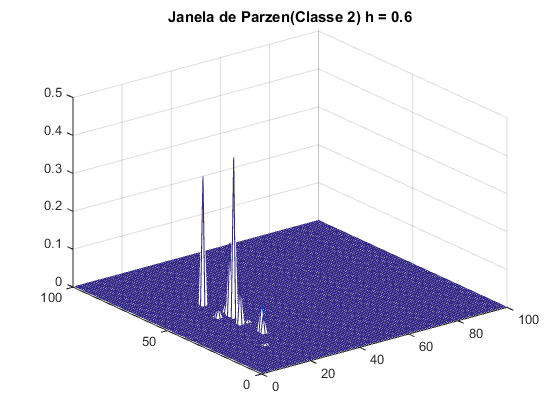
\includegraphics[scale=0.75]{parzen_c2_h06}
    \caption{}
    \label{fig:parzen_c2_h06}
\end{figure}


\section*{Letra C}

O código \code{kNN.py} implementa a probabilidade \emph{a posteriori} de $\omega_i$
em relação a uma amostra $\mathbf{x}$. Como demonstrado em \autocite{duda.hart.stork.2000},
uma boa estimativa de $P(\omega_i|\mathbf{x})$ é

\begin{equation}
P_n(\omega_i|\mathbf{x}) = \frac{p_n(\mathbf{x}, \omega_i)}{\sum_{j=1}^c p_n(\mathbf{x}, \omega_j)}
\label{eq:prob_posteriori}
\end{equation}

\noindent e como

\begin{equation}
p_n(\mathbf{x}, \omega_i) = \frac{k_i / n}{V}
\label{eq:dens_prob_conjunta}
\end{equation}

e

\begin{equation}
\sum_{j=1}^c k_j = k
\label{eq:sum_k_i}
\end{equation}

\noindent então \equationref{prob_posteriori} torna-se

\begin{equation}
P_n(\omega_i|\mathbf{x}) = \frac{k_i}{k}
\label{eq:prob_posteriori_2}
\end{equation}

A equação descrita acima apenas demonstra que $P_n(\omega_i|\mathbf{x})$ tende a
$P(\omega_i|\mathbf{x})$ quando $k$ cresce. Logo, achando os $k$ vizinhos mais
próximos ao ponto $\mathbf{x}$ temos o valor estimado de sua probabilidade
\emph{a posteriori}. \figureref{kNN-k9-P_w1_given_x} e \figureref{kNN-k9-P_w2_given_x}
mostram as estimações para $k = 9$. Note que o gráfico de $\omega_1$ é o inverso
do de $\omega_2$. Isto ocorre porque

\begin{equation}
P_n(\omega_1|\mathbf{x}) + P_n(\omega_2|\mathbf{x}) = 1
\label{eq:sum_prob_posteriori}
\end{equation}

\begin{figure}[ht]
    \centering
    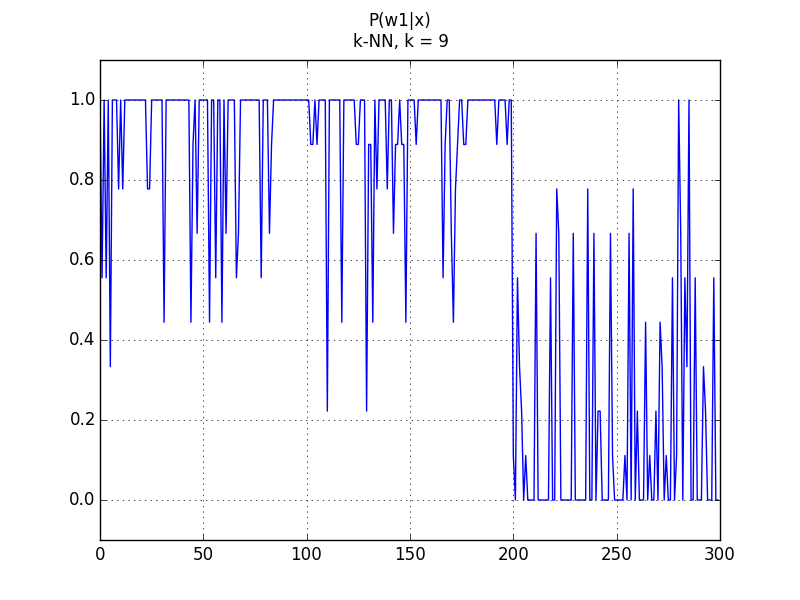
\includegraphics[scale=0.75]{kNN-k9-P_w1_given_x}
    \caption{}
    \label{fig:kNN-k9-P_w1_given_x}
\end{figure}

\begin{figure}[ht]
    \centering
    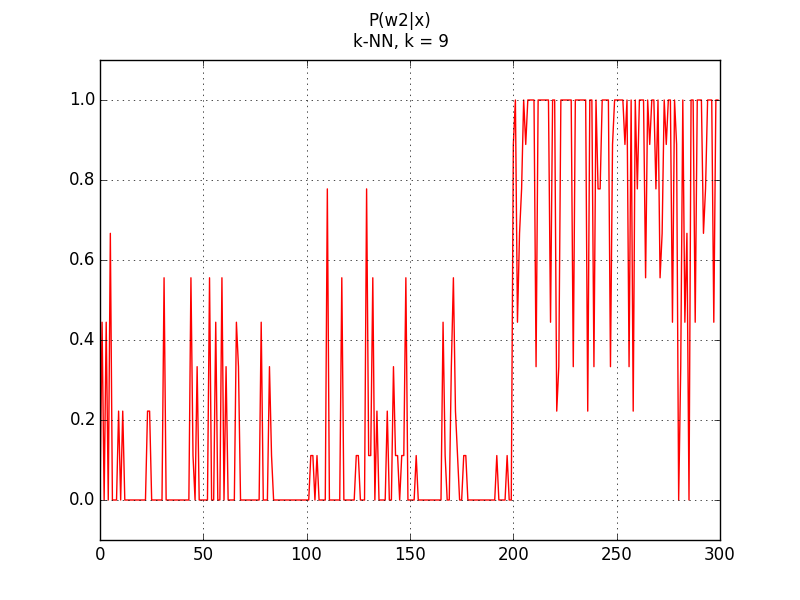
\includegraphics[scale=0.75]{kNN-k9-P_w2_given_x}
    \caption{}
    \label{fig:kNN-k9-P_w2_given_x}
\end{figure}


\section*{Letra D}

Utilizando um MLP treinado com backpropagation obtemos através de \code{MLP.m} um
erro médio quadrático convergente após 300 épocas. O algoritmo permanece em execução
até 10000 épocas (\figureref{mse_x_epochs}). Foram usadas 3 camadas escondidas e
o resultado da classificação foi documentado em \emph{mlpout.txt}, onde a primeira
coluna corresponde aos objetos da classe 1 e 2, respectivamente, na mesma ordem
das matrizes r11, r12 e r2. A segunda coluna corresponde a saída da rede neural
e a terceira, ao erro. Considerou-se que a classe 2 deve ter resposta ideal zero
e a classe 1, deverá ter resposta 1.

\begin{figure}[ht]
    \centering
    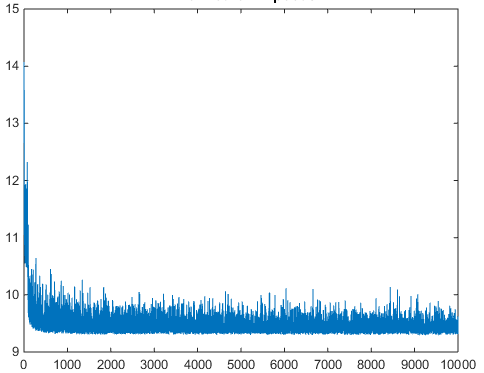
\includegraphics[scale=0.75]{mse_x_epochs}
    \caption{}
    \label{fig:mse_x_epochs}
\end{figure}


\section*{Letra E}

A regra da soma, implementada em \code{regra\_soma.m}, para uma determinada classe
$\omega_j$ é dada por

\begin{equation}
(1 - L) P(\omega_j) + \sum_{i=1}^L p(\omega_j|\mathbf{x_i})
\label{eq:sum_prob_posteriori}
\end{equation}

\begin{figure}[ht]
    \centering
    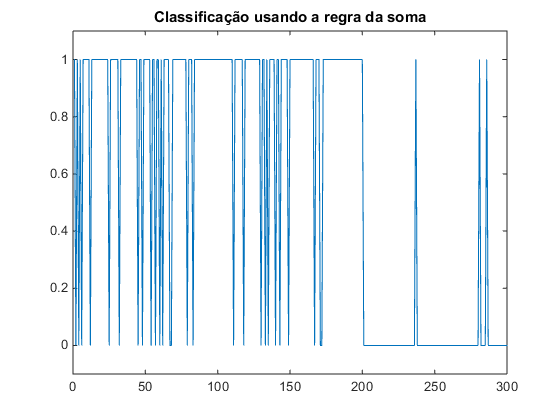
\includegraphics[scale=0.75]{sum_rule}
    \caption{}
    \label{fig:sum_rule}
\end{figure}


\printbibliography

\end{document}